\documentclass[../main]{subfiles}
\ifSubfilesClassLoaded{
    \dominitoc
    \tableofcontentsfile
	\pagenumbering{arabic}
    \setcounter{page}{1}
}{}

\begin{document}
\graphicspath{{06-Analyse/figures},{../06-Analyse/figures}, {../06b-Analyse-2D}}

\chapter{Extension aux cartes en deux dimensions}

\minitoc
Nous avons étudié des comportements de base de cartes 1D sur des données en une dimension. 
Cependant, les cartes auto-organisatrices utilisées en pratique sont des cartes en deux dimensions, qui permettent bien mieux de cartographier des données en grande dimension.
Ce chapitre présente une étude préliminaire d'architectures de deux et trois cartes en deux dimensions. 
Nous cherchons à étudier ici si les mécanismes d'organisation observés sur des cartes 1D sont transposables à des cartes en deux dimensions et dans quelle mesure. Ceci nous permettra d'identifier les limites et perspectives du passage des cartes 1D à 2D.

\section{Jeu d'entrées géométriques en grande dimension}

Maintenant que nous travaillons sur des cartes en deux dimensions, nous voulons que chaque carte prenne des entrées de dimension supérieure ou égale à deux. Nous nous concentrons dans ce chapitre sur des cartes prenant des entrées 2D, dans un cas géométrique similaire aux cartes 1D du chapitre précédent prenant des entrées unidimensionnelles.
Les entrées multimodales sont donc des points en 4 dimensions pour une structure de 2 cartes.
Nous choisissons ces points sur une sphère en 3D dont on a effectuée une rotation dans l'espace 4D, de la même façon que les entrées en 3D se trouvaient sur un cercle 2D dont on a effectué une rotation dans l'espace, voir figure~\ref{fig:sphere_inputs}. 
La variable $U$ paramétrant cette surface est alors en deux dimensions et permet de représenter le modèle d'entrées.
Nous normalisons les entrées entre 0 et 1 sur chaque dimension, entrainant une légère déformation de la sphère.

Nous nous intéressons à une architecture de deux cartes 2D.
Chaque carte possède une couche de poids externes  $\w\ext \in [0,1]^2$ et une couche de poids contextuels $\w_c \in [0,1]^2$.
Les BMUs de chaque carte sont indexés par des positions en deux dimensions $\bmu = (\bmu_0, \bmu_1)$. 
Nous prenons des cartes  de taille $100x100$.
Les activités $a_e$ et $a_c$ sont calculées par une activitation gaussienne: 
$$a_e(\inpx,p) = \exp(\frac{||\inpx - \w_e(p) ||^2}{2*\sigma^2})$$
, identiquement pour $a_c$. La norme utilisée dans les cartes 2D est la norme euclidienne.

\begin{figure}
	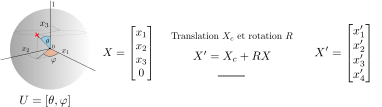
\includegraphics[width=\textwidth]{sphere_inputs.pdf}
	\caption{Transformation d'une surface d'un espace 3D en surface dans un espace 4D ou 6D. Les points restent positionnés sur une surface, mais sont plongés dans un espace de plus grande dimension. La rotation permet de répartir les coordonnées des points sur les dimensions. \label{fig:sphere_inputs}}
\end{figure}

\section{Organisation des poids}

La notion d'organisation dans une carte 2D est moins directe que dans une carte en une dimension.
De plus, l'organisation des poids externes n'est pas forcément assurée pour un rayon de voisinage constant, même dans une carte sans connexions contextuelles. Par exemple, l'organisation attendue d'une carte sur le carré $[0,1]^2$ est que les coins de la carte viennent dans les coins du carré. Cependant, les mécanismes d'organisation peuvent conduire à une carte tordue en son milieu, par exemple en \label{fig:torsion}.

\begin{figure}
	\centering\includegraphics[width=0.7\textwidth]{we_cub_example.pdf}
	\caption{Exemple de point de torsion dans une carte 2D dépliée sur des entrées dans $[0,1]^2$ (B). La carte A au contraire est bien dépliée~: deux entrées proches sont représentées par des BMUs proches. Cette disposition présentant un point de torsion peut évoluer vers une carte bien dépliée ou vers un état stable présentant un point de torsion, en fonction des paramètres d'apprentissage. \label{fig:torsion}
	}
\end{figure}

Dans une architecture CxSOM, cela peut poser un problème pour l'utilisation de la position du BMU en tant que représentation de l'entrée~: la position du BMU n'est plus directement représentative de l'entrée. Deux entrées proches peuvent avoir leur BMU de chaque côté de la carte.
Dans un premier temps, nous avons choisi de forcer les cartes à bien se déplier . Pour cela, nous laissons les poids externes s'organiser sur quelques centaines d'itérations, préalablement aux poids contextuels, en prenant un grand rayon de voisinage $r_e = 0.5$. 
Ce grand rayon permet d'éviter les zones de torsion dans la carte. Après cette étape préalable, nous réduisons le rayon externe  à $r_e = 0.2$ et effectuons l'apprentissage des poids externes et contextuels comme décrit dans le modèle CxSOM. Les poids externes affinent alors leur apprentissage et les poids contextuels s'organisent sur une carte "bien dépliée". 
La généralisation de l'organisation des architectures 2D serait à explorer pour assurer une robustesse de l'algorithme sur des données quelconques~: il est en effet compliqué de s'assurer du bon dépliement d'une carte en pratique sur des données de grande dimension.

\subsection{Organisation de cartes sur des entrées indépendantes}

Intéressons nous à l'organisation d'une architecture de deux cartes prenant des entrées $\inpx\m{1}, \inpx\m{2} \in [0,1]^2 \times 0,1]^2$ indépendantes. Nous prenons des rayons de voisinage $r_e = 0.2, r_c = 0.05$.
Dans l'architecture de cartes 1D, l'apprentissage sur des données indépendantes conduit à la formation de zones dans les poids contextuels de chaque carte. Nous voulons vérifier si la présence de telles zones est observable sur des cartes 2D.
Nous nous intéressons d'abord aux motifs formés par les poids externes et contextuels sur chaque carte.

Les valeurs des poids externes et contextuels sont tracés en figure \ref{fig:2som_cub_wc}.
Nous traçons les poids externes des cartes dans l'espace des entrées~: chaque point $p$ de la carte est positionné en $\w_e(p)$ et relié à ses voisins pour représenter le voisinage.
Nous utilisons une représentation à l'aide d'une carte de coloration pour les poids contextuels. Le pixel situé à la position $p$ sur l'image prend la couleur correspondant à la valeur de son poids contextuel $w_c$, définie par la carte de coloration tracée à droite sur la figure.


Cette représentation permet de faire apparaître clairement des motifs dans la disposition des poids.
Tracer les poids nous permet ici de comparer l'organisation d'une carte à celle observée en une dimension. Nous soulignons cependant que cette représentation ne permet pas de détecter quelles unités sont effectivement BMU lors d'un test.
Les poids externes sont ici bien dépliés sur l'ensemble des entrées, ce qui est similaire au cas en une dimension.
Les poids contextuels font apparaître des motifs dans leur disposition. 
Les motifs sont similaires sur les deux cartes, traduisant un aspect systématique et non aléatoire.
En traçant l'organisation des poids pour des cartes de paramètres $r_c$ différents, nous remarquons également que l'échelle des motifs dépend de la valeur du rayon de voisinage contextuel, comme dans le cas en une dimension.
Néanmoins, les poids restent centrés autour de $0.5$~: nous faisons apparaître en bleu et orange sur la carte de coloration les valeurs effectivement prises par les poids contextuels de chaque carte. 
Pourtant, les positions des BMUs de chaque carte observées lors d'un test s'étendent bien sur toute la surface d'une carte. Les poids contextuels auraient dû, pour bien cartographier les positions sur l'autre carte, s'étendre sur tout le carré dans chaque zone.
Ce comportement est à voir comme une limite des architectures de cartes, mais cette limitation est générale à des cartes une et deux dimensions~:  Des architectures de 10 cartes apprenant sur 10 entrées 1D indépendantes voient également leurs poids contextuels se moyenner autour de 0.5.

\begin{figure}
	\begin{minipage}{\textwidth}
		\centering\includegraphics[width=0.6\textwidth]{we_cub_example.pdf}
	\end{minipage}
	\begin{minipage}{\textwidth}
		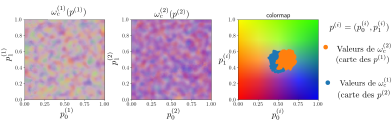
\includegraphics[width=\textwidth]{wc_cub_legend.pdf}
		\caption{En haut: poids externes des cartes $M\m{1}$ et $M\m{2}$ représentés sous forme de distorsion de la carte après 200000 itérations.
	En bas: poids contextuels des cartes pour la même itération, représentés sous forme de carte de couleur en deux dimensions. Un pixel situé à la position $p_i,p_j$ prend comme couleur correspondante la valeur 2D de son poids contextuel, associé à une couleur par la carte de coloration représentée à droite de la figure.
	Les points orange et bleus indiqués sur la carte de coloration sont les valeurs effectivement prises par toutes les valeurs de $\w_c^{(1)}$ et $\w_c^{(2)}$, cartographiant les positions des BMUs de l'autre carte.
	On remarque donc que les poids contextuels ne se déplient pas sur toutes les valeurs prises par les BMUS, car toutes les unités de la carte ont été BMU lors de cette phase de test.\label{fig:2som_cub_wc}}
	\end{minipage}
\end{figure}


\subsection{Organisation des cartes sur des entrées dépendantes}

Nous étudions l'organisation des cartes sur des données pris sur une sphère 3D, tournée dans un espace en 4D. Les données ont ici deux degrés de liberté qui sont les angles paramétrant la représentation polaire de la sphère.
Nous prendrons dans une première expérience les paramètres $r_c = 0.02$ et $r_e = 0.2$.
La figure~\ref{fig:2som_s_002_wc} présente la disposition des cartes après 700 000 itérations d'apprentissage. 

Cette configuration de poids est stable~: seule une zone réduite de la carte évolue encore après les 700000 itérations, sur un cycle limite restreint en termes de valeurs. 
On peut donc parler ici de convergence.
Les poids externes cartographient les entrées externes de la même façon qu'une carte indépendante, ce qui est bien attendu du modèle CxSOM. Chacune des carte s'étend sur le cercle dans lequel sont tirées leurs entrées externes.
Les poids contextuels de la carte, représentés sous forme de carte de coloration, font apparaître des motifs alternés.
Ces motifs rappellent bien les motifs présents en une dimension en faisant alterner des valeurs opposées (rouge et vert).
Le tracé des entrées en fonction de la position du BMU fait également figurer l'existence de zones mortes de taille réduite.


Une première différence avec les cartes en une dimension est la forme des zones, moins régulières. Ces zones semblent dépendre des paramètres choisis.
Nous comparons en Figures~\ref{fig:rc_003,fig:rc_005} et \ref{fig:todo} l'évolution des poids contextuels au cours de l'apprentissage pour une même distribution de données d'entrées et $r_c = 0.05, 0.03$ et $0.02$
Nous remarquons que l'expérience avec $r_c = 0.02$ conduit à une configuration stable des poids contextuels, dont certains ont convergé vers un point fixe et d'autres vers un cycle limite, comme l'indique la figure TODO. Cette convergence est également assurée dans l'expérience avec $r_c = 0.03$. Au contraire, les poids contextuels ne montrent pas de convergence pour $r_c =0.05$. Nous avons observé expérimentalement ce comportement sur plusieurs expériences.

Cependant, nous observons une organisation des poids contextuels similaires dans ces trois expériences, ce qui montre que les motifs dépendent bien de la relation entre entrées et non des conditions initiales des expériences. 
Nous remarquons en effet que les poids contextuels tendent à s'organiser sous une forme hélicoïdale, formant les motifs observé dans les trois expériences.
La dynamique de l'évolution des poids au cours de l'apprentissage suit par ailleurs cette forme d'hélice. 
Les zones "floues" observées dans les poids contextuelles correspondent aux zones de transition

Nous pouvons conclure de ces observations préliminaires en deux dimensions que la formation de zones est un mécanisme qu'on retrouve dans des cartes 1D comme des cartes 2D. Cependant, les deux dimensions apportent beaucoup moins de contraintes sur la forme des zones que sur des cartes en une dimension, rendant possible la formation différents motifs sur les poids contextuels. 
Contrairement au cas en une dimension dans lequel la convergence des poids était assurée, la convergence des poids contextuels dans une carte 2D n'est pas assurée en fonction des paramètres de la carte. Cette étude paramétrique en deux dimensions apparaît comme une suite nécessaire de l'étude des cartes.

Nous avons analysé la forme des poids sur un seul type de distribution, une sphère dans un espace 4D, pour différents rayons de voisinage de la carte.
Nous observons que les motifs formés par les poids contextuels sont similaires dans tous ces cas et ne dépendent donc pas des conditions initiales des expériences~: les poids des cartes sont initialisés aléatoirement de façon différente dans chaque expérience et les entrées sont tirées sur une même distribution de façon aléatoire.
Nous pouvons donc supposer que le type de relation entre entrées influence ces motifs. L'étude des comportements d'une carte 2D en fonction du type entrées est une suite pertinente de ces résultats préliminaires.


\begin{figure}
	\begin{minipage}{\textwidth}
		\centering\includegraphics[width=0.6\textwidth]{2SOM_sphere_we_249999.pdf}
	\end{minipage}
	\begin{minipage}{\textwidth}
		\centering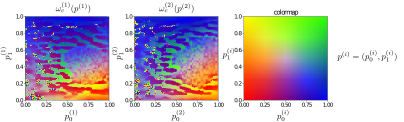
\includegraphics[width=\textwidth]{wc_s_002_legend.pdf}
		\caption{Tracé des poids contextuels d'une architecture de cartes, organisées sur une sphère dans un espace 4D, avec $r_e =0.2$ et $r_c = 0.02$. Contrairement au cas avec $r_c = 0.05$ précédemment tracé, les poids contextuels atteignent un état stable~: ils sont fixes dans toute la carte et sont dans un cycle limite dans la "tâche". Les motifs ne sont donc pas déterminés par les poids mais plutôt par les conditions initiales et l'évolution de la carte. Nous remarquons que les valeurs de $\w_c$ dans chaque carte se déplient bien ici sur toutes les valeurs prises par les BMU.
		\label{fig:2som_s_002_wc}}
	\end{minipage}
\end{figure}


\begin{figure}
	\includegraphics[width=\textwidth]{sphere_rc005_evol_landscape}
	\caption{Evolution des poids contextuels d'une architecture de deux cartes pour $r_c =0.05$. Les points sont représentés sous forme de carte de coloration à gauche et sous forme de disposition dans l'espace des positions sur la figure de droite. On observe une évolution régulière sous forme de motif en hélice, mais cette disposition évolue dans le temps. Après 700000 itérations, la figure semble se déformer vers de nouveaux motifs. Cette organisation ne converge pas. Les valeurs prises par les poids contextuels des cartes $M\m{1}$ (bleu) et $M\m{2}$ (orange) sont tracés sur la carte de coloration, faisant apparaître un motif hélicoïdal évoluant dans le temps.
	\label{fig:rc_005}}
\end{figure}


\begin{figure}
	\includegraphics[width=\textwidth]{wc_rc003_evol.pdf}
	\caption{\'Evolution des poids contextuels d'une architecture de deux cartes pour $r_c =0.03$. Les motifs observés sont similaires à ceux observés pour d'autres paramètres. Les poids présentent toujours une forme hélicoïdale évoluant dans le temps.\label{fig:rc_003}}
\end{figure}

\begin{figure}
	\includegraphics[width=\textwidth]{wc_rc002_evol.pdf}
	\caption{\'Evolution des poids contextuels d'une architecture de deux cartes pour $r_c =0.02$. Les motifs observés sont similaires à ceux observés pour d'autres paramètres. Les poids présentent toujours une forme hélicoïdale évoluant dans le temps. \label{fig:rc_002}}
\end{figure}



%CONVERGENCE RELAX ! 

\subsection{Convergence de la relaxation}

Nous traçons enfin en figure \label{fig:relax} l'évolution du taux de convergence des tests au cours de l'apprentissage pour des structures de deux cartes en deux dimensions, par le
processus décrit au chapitre \ref{chap:relax}.
Des phases de test sont lancées à intervalles réguliers au cours de l'apprentissage. Lors de chaque test, nous comptons le nombre de pas de relaxation nécessaires à la convergence. Nous traçons sur la figure la moyenne de ces pas de relaxation sur chaque test $t$. 
Nous traçons également sur la deuxième figure le taux d'échantillons menant à une convergence de la relaxation. On considère que la relaxation n'a pas convergé si le nombre de pas est de 1000, seuil maximal fixé par notre étude. Le nombre de pas de relaxation moyen étant de 20 pas, ce seuil est pertinent. 
Ces tracés ont été réalisés sur trois expériences de mêmes paramètres $r_e=0.2$ et $r_c = 0.02$.
Nous y faisons figurer l'évolution du nombre moyen de pas et du taux de convergence pour l'expérience avec $r_c = 0.05$. Dans cette expérience, les poids n'ont pas formé de zones distinctes et ne convergence pas vers une valeur fixe.
Nous voyons que la relaxation converge bien dans tous les cas. Le nombre moyen de pas de relaxation tourne autour de 50 et entre 95 et 98 \% des recherches de BMU par relaxation convergent dans chaque expérience. 
Les valeurs trouvées pour $r_c = 0.05$ sont similaires au cas $r_c = 0.02$, dans lequel les poids ont bien convergé. La relaxation n'est donc pas tributaire de la formation de zones stables.

Cette observation est prometteuse pour la construction d'architectures. Cela montre que le BMU a un sens dans une carte en deux dimensions. 
Nous n'avons pas étudié en deux dimensions l'unicité du BMU en fonction des valeurs d'initialisation de la relaxation. Nous avons cependant observé que la relaxation converge la plupart du temps, et qu'elle converge vers une valeur dont le poids $\w_e(\bmu)$ est proche de l'entrée externe. Cela suffit pour considérer que le BMU a bien un sens en terme d'apprentissage.

\begin{figure}
	\centering
	\includegraphics[width=0.7\textwidth]{conv_relax_2maps.pdf}
	\caption{\'Evolution de la convergence de la relaxation au cours de l'apprentissage. Nous avons réalisé les tracés sur trois expériences générées pour $r_c = 0.02$, sur des entrées aléatoires tirées sur la même distribution, une sphère 4D. Pour comparaison, nous traçons également l'évolution pour l'expérience avec $r_c = 0.05$, dans laquelle les poids contextuels n'ont pas convergé. La relaxation converge en fin d'apprentissage~: le BMU a donc un sens dans les cartes en deux dimensions. \label{fig:relax}}
\end{figure}

\section{Prédiction d'entrée}

Nous avons vu que les cartes en deux dimensions s'organisent, comme en 1D, de manière à former des zones dans les poids contextuels. 
Nous avons également observé que la recherche de BMU a un sens, car la relaxation converge dans les cartes 2D.
Nous nous attendons donc à ce qu'une architecture de cartes 2D soit en mesure de générer une prédiction.

Pour cela, nous construisons une architecture de trois cartes en deux dimensions. Chaque carte prend en entrée externe une paire de coordonnées d'un espace multimodal en 6D. Ces entrées sont situées sur une sphère de dimension 3 plongée dans l'espace en 6D. $U$ est donc une variable $2D$. 
Dans cette configuration, la connaissance de deux entrées sur trois et du modèle détermine la troisième~: la prédiction est donc possible.
Nous prenons $r_e = 0.2$ et $r_c = 0.02$, pour des cartes de taille $100 \times 100$. Les cartes sont entraînées sur 250 000 itérations, à l'issue desquelles les poids contextuels ont atteint une position stable.


Nous traçons d'abord les poids externes et contextuels des trois cartes sont représentés en Figure~\ref{fig:3som_w}.
L'organisation des poids contextuels conduit à la présence de motifs très semblables à ceux observés sur une architecture de deux cartes.

Nous lançons une étape de prédiction à la fin de l'apprentissage lors de laquelle la carte $M\m{1}$ ne reçoit plus d'entrée externe. 
La valeur de $\w\ext\m{1}(\bmu\m{1})$ est alors utilisée comme prédiction de l'entrée $\inpx\m{1}$.
La Figure~\ref{fig:3som_pred} indique la valeur prédite en fonction de l'entrée $\inpx\m{1}$. 
Les valeurs de $\inpx$ et $\w_e$ étant 2D, nous avons représenté séparément chaque dimension. 
Les tracés montrent que la prédiction est bien réalisée.

La capacité de prédiction observée dans le cas 2D est prometteuse et nous montre que l'architecture de cartes ont bien appris le modèle d'entrées 2D.

\begin{figure}
	\begin{minipage}{\textwidth}
		\centering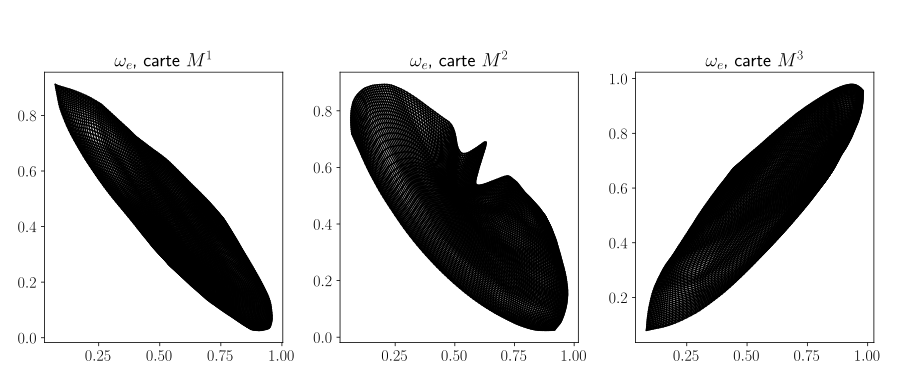
\includegraphics[width=0.7\textwidth]{3SOM_S_we_239999.pdf}
	\end{minipage}
	\begin{minipage}{\textwidth}
		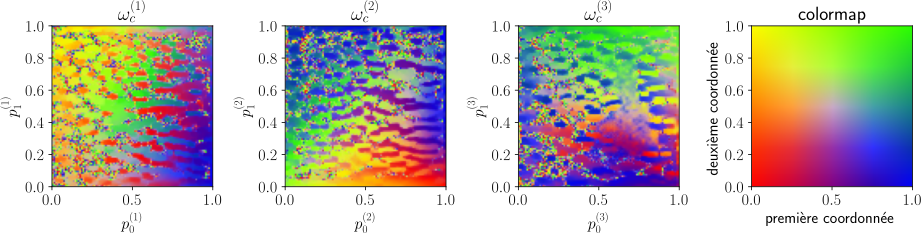
\includegraphics[width=\textwidth]{3SOM_S_wc_239999.pdf}
		\caption{\label{fig:3som_w}}
	\end{minipage}
\end{figure}

\begin{figure}
\includegraphics[width=0.7\textwidth]{zclosed-1-239999_error.pdf}
\caption{Tracé de l'erreur de prédiction $\w_e\m{1}(X\m{1})$ en fonction de la valeur théorique de $X^{(1)}$, non présentée à l'architecture, dans une architecture de trois cartes 2D prenant des entrées $X^{(i)}$ en deux dimensions $[X^{(i)}_0, X^{(i)}_1]$. Nous traçons sur une ligne, pour chaque entrée, les dépendances entre chacune des dimensions.
Lorsque la carte $M^{(1)}$ ne reçoit pas d'entrée externe. Les cartes $M^{(2)}$ et $M^{(3)}$ ayant une activité externe, le graphique montre que la quantification vectorielle est bien réalisée dans ces cartes. La carte $M^{(1)}$ est uniquement activée par les connexions contextuelles venant de $M^{(2)}$ et $M^{(3)}$. La figure du haut montre que la prédiction est correctement réalisée.\label{fig:3som_pred}}
\end{figure}



\section{Limites et perspectives}




\subsection{Perspectives}
%Convergence des cartes 2D Cottrell 

\section{Conclusion}


\ifSubfilesClassLoaded{
    \printbibliography
    %\externaldocument{../main.tex}   
}{}
\end{document}



% PLAN


% Convergence des poids :
% - Dépend des paramètres, contrairement à la carte en 1D on n'arrive pas forcément dans une position stable
% - Rc = 0.02 : point fixe, avec une partie 
% - Chaque expérience différente : grande dépendance aux conditions initiales. 